\documentclass{supervision}
\usepackage{course}
\usepackage{fancyvrb}
\usepackage{qtree}

\Supervision{3}
\Topics{Colour, displays and image processing}

\begin{document}

\section*{From Supervision 2}
\begin{questions}
  \question Derive the conditions necessary for two Bézier curves to join with:
    \begin{solution}
      Consider two bezier curves $p(t)$ and $q(t)$, defined by control points
      $(p_0,p_1,..., p_n)$ and $(q_0, q_1,..., q_n)$ respectively.
    \end{solution}
  \begin{parts}
    \part just C0-continuity
      \begin{solution}
        $C0$ continuity can be achieved by setting $p(1) = q(0)$ giving:
        \begin{center}
          $q_0 = p_n$
        \end{center}
      \end{solution}
    \part C1-continuity
      \begin{solution}
        $C1$ continuity can be achieved with the additional constraint that
        $p'(1) = q'(0)$ giving:
        \begin{center}
          $q_1 - q_0 = p_n - P_{n-1}$
        \end{center}

        Which when combined with the above constraint gives:
        \begin{center}
          $q_1 = 2p_n - p_{n-1}$
        \end{center}
      \end{solution}
    \part C2-continuity
      \begin{solution}
        For $C2$ continuity we must also have that $p''(1) = q''(0)$, giving:
        \begin{center}
          $q_2 - 2q_1 + q_0 = p_n - 2P_{n-1} + p_{n-2}$
        \end{center}

        Which when combined with the above constraint gives:
        \begin{center}
          $q_2 = p_{n-2} + 4(p_n - p_{n-1})$
        \end{center}
      \end{solution}
  \end{parts}

  \question What would be difficult about getting three Bézier curves to join
    in sequence with C2-continuity at the two joins?
    \begin{solution}
      Control points would be dependant on two other curves?
    \end{solution}

  \question
    For a cylinder of radius $2$, with endpoints $(1,2,3)$ and $(2,4,5)$, show
    how to calculate:
    \begin{parts}
      \part an axis-aligned bounding box
        \begin{solution}
          Let $m$, $n$, and $o$ represent the $x$, $y$, and $z$ axes
          respectively.

          Let $A$ and $B$ be the endpoints such that $A_M <= B_M$.

          Let $
          \delta =
          \frac{\sqrt{(A_n - B_n)^2 + (A_o - B_o)^2}}
               {(A_m - B_m)^2 + (A_n - B_n)^2 + (A_o - B_o)^2}
          $

          $m_{min} = A_m - \delta \times r$ \\
          $m_{max} = B_m + \delta \times r$


        \end{solution}

      \part a bounding sphere
        \begin{solution}
          \begin{center}
            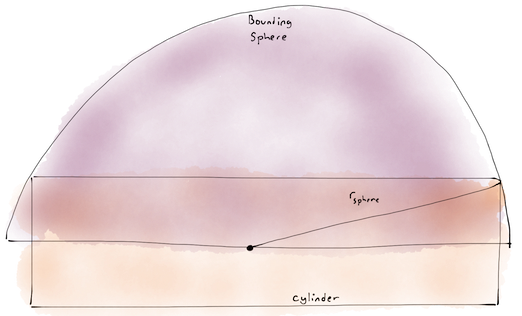
\includegraphics[width=0.5\textwidth]{3-3-bounding-sphere}
          \end{center}
          The bounding sphere has midpoint that is half way between the two
          endpoints:
          ${mid} = (1.5, 3, 4)$

          The radius is the distance from the midpoint to a point on the edge
          of the cylinder.

          One such point is $(2, 4 + \sqrt{2}, 5 - \sqrt{2})$.

          Giving: $r = \sqrt{(0.5)^2 + (1+\sqrt{2})^2 + (1-\sqrt{2})^2} = 2.5$
        \end{solution}
    \end{parts}

  \question Break down the following (2D!) lines into a BSP-tree, splitting
    them if necessary:
    \begin{description}
      \item[a] $(0,0)-( 2,2)$
      \item[b] $(3,4)-( 1,3)$
      \item[c] $(1,0)-(-3,1)$
      \item[d] $(0,3)-( 3,3)$
      \item[e] $(2,0)-( 2,1)$
    \end{description}
    \begin{solution}
      \begin{center}
        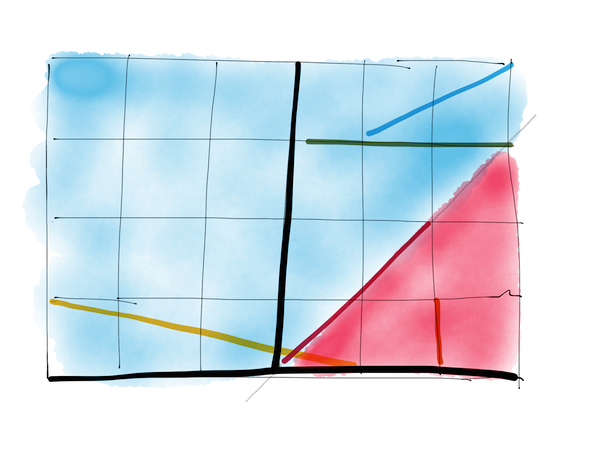
\includegraphics[width=0.5\textwidth]{3-4-bsp}
      \end{center}
      \Tree[.a
        [.d b   c_1 ]
        [.e c_2     ]
      ]
    \end{solution}

  \question
    \begin{parts}
      \part Compare the two methods of doing 3D clipping in terms of
        efficiency
        \begin{solution}
          \emph{Not sure which is more efficient - both require clipping
          against 6 axes.}
        \end{solution}
      \part How would using bounding volumes improve efficiency of these
        methods?
        \begin{solution}
          Computing and storing bounding volumes for each object in the scene
          makes it much easier to quickly determine that two objects don't
          intersect.
        \end{solution}
    \end{parts}

  \question Describe a complete algorithm to do 3D polygon scan conversion,
    including details of clipping, projection, and the underlying 2D polygon
    scan conversion algorithm.
    \begin{solution}

      \begin{lstlisting}[gobble=8]
        class Screen():
          def __init__(self, x=1920, y =1080):
            self.x = x
            self.y = y
          def get_pixels(self):
            for x in range(0, self.x):
              for y in range(0, self.y):
                yield (x,y)

        class Polygon():
          get_pixels():
            # projects the polygon to 2D and runs 2D polygon scan-conversion

        for (x,y) in screen.get_pixels():
          color[x][y] = background_color
          depth[x][y] = infinity

        for polygon in scene:
          for (x,y) in polygon.get_pixels():
            if polygon.depth(x,y) < depth[x][y]:
              depth[x][y] = z
              color[x][y] = polygon.color(x,y)
      \end{lstlisting}

      % TODO
    \end{solution}

  \question Describe how you would form a good approximation to a cylinder
    from Bézier patches. Draw the patches and their control points and give
    the coordinates of the control points.
    \begin{solution}
      \emph{Not sure why you can't just use two bezier patches, one for each
      side of the cylinder (although this doesn't do the top).}
    \end{solution}

  \question Given the following sixteen points, calculate the first eight of
    the next patch joining it as $t$ increases so that the join has continuity
    $C1$. Here the points are listed with $s=0$, $t=0$ on the bottom left,
    with $s$ increasing upwards and $t$ increasing to the right:
    \begin{Verbatim}[fontsize=\scriptsize]
(-0.2, 3.4,  0.3)    (1.0, 3.1, 0.2)    (2.0, 2.6, -0.2)    (3.1, 2.8,  0.2)
( 0.0, 1.2,  0.4)    (1.2, 2.0, 1.2)    (1.4, 1.9, -0.2)    (2.7, 1.8,  0.2)
( 0.2, 1.0, -0.2)    (1.1, 0.8, 0.5)    (1.4, 1.0,  0.0)    (3.1, 1.1, -0.2)
( 0.0, 0.0,  0.0)    (1.0, 0.0, 0.5)    (2.0, 0.2,  0.4)    (2.7, 0.0, -0.2)
    \end{Verbatim}
    \begin{solution}
      \begin{Verbatim}[fontsize=\scriptsize]
(3.1, 2.8,  0.2)    (4.2,  3.0,  0.6)
(2.7, 1.8,  0.2)    (4.0,  1.7,  0.6)
(3.1, 1.1, -0.2)    (4.8,  1.2, -0.4)
(2.7, 0.0, -0.2)    (3.4, -0.2, -0.8)
      \end{Verbatim}
    \end{solution}
\end{questions}

\section*{\Topics}
\subsection*{Warmup Questions}
\begin{questions}
  \question Compare and contrast the use of LCDs and electrophoretic displays
    for screens in portable devices.
    \begin{solution}
      LCDs are more common in mobile devices as they can produce a wide
      variety of colours and are thus suitable for the rich interface on
      mobile phones and tablets.

      Electrophoretic displays are typically used in e-book readers as it is
      easier to read for extended periods of time from an electrophoretic
      display than an LCD display. They also have the benefit that power is
      only required to change the display which means the e-book reader can
      have a long battery life as changing the display is not a frequent
      operation.

      LCDs have a faster refresh rate than e-ink displays and a higher pixel
      density, and due to the backlight can be seen in darkness (although some
      e-ink displays do now have backlights).
    \end{solution}

  \question Compare the rendering in some different pieces of printed
    material. Use a magnifying glass to explore the resolution, colours and
    patterns used.

\end{questions}

\subsection*{Longer Questions}
\begin{questions}
  \question Explain the use of each of the following colour spaces:
    \begin{parts}
      \part $RGB$
        \begin{solution}
          The standard RGB colour space was created for use on monitors and
          the internet. Since displays use red, green, and blue LEDs to create
          light it suits this application well.
        \end{solution}
      \part $XYZ$
        \begin{solution}
          The first attempt to produce a colour space based on measurements of
          human colour perception and it is the basis for almost all other
          colour spaces.
        \end{solution}
      \part $HSL$
        \begin{solution}
          Used by artists as it is more natural to think about a colour in
          terms of hue and saturation rather than additive or subtractive
          colour components.
        \end{solution}
      \part $LUV$
        \begin{solution}
          It is used in computer graphics when dealing with coloured lights.
          Additive mixtures of different colours will not fall along a line in
          the ${LUV}$ colour space unless the mixtures have the same lightness.
        \end{solution}
    \end{parts}
  \question Explain the difference between additive colour (${RGB}$) and
    subtractive colour (${CMY}$). Where is each used and why is it used there?
    \begin{solution}
      Additive colour is good when dealing with light as that is how
      combinations of light sources behave. Subtractive colour is used when
      dealing with the colour of an object as this works by absorbing light.
    \end{solution}

  \question Compare the two methods of \emph{Error Diffusion} described in the
    notes, with the aid of a sample image.
    % TODO

\end{questions}
\end{document}
